% INTRODUCTION
Marine aggregates are randomly formed particles composed of organic and inorganic matter, such as phytoplankton, detritus, sediment, and fecal pellets~\cite{jackson_simulation_1989}. Since these components stick together arbitrarily, a marine aggregate is often shown as a fractal structure. 
These marine aggregates take in carbon dioxide (CO$_2$) during photosynthesis near the surface ocean and carry the dissolved carbon to the deep ocean. 
% The ocean absorbs $40 \%$ of the anthropogenically produced carbon dioxide (CO$_2$) from the atmosphere~\cite{omand_sinking_2020}. 
This process removes CO$_2$ from the atmospheric carbon cycle~\cite{honjo_understanding_2014} and plays a role in regulating atmospheric CO$_2$ and climate changes which is one of the most significant environmental problems we face today. 
 \par
 It has been observed that larger sinking aggregates tend to accumulate in thin layers where the ambient fluid is density stratified~\cite{alldredge_occurrence_2002}. The highly concentrated thin layers become biological hotspots for bacterial activity and animal feeding. It is ecologically important to understand the marine aggregates' dynamics as they delay in settling.
\par
We consider flows around aggregates in the low Reynolds number regime, which is applicable for approximately the smallest 30\% of marine aggregates~\cite{alldredge_situ_1988}. Flow in this regime is governed by the Stokes equations, which allows solutions to be found via boundary integral methods~\cite{pozrikidis_boundary_1992}. Such methods have been implemented in several different contexts, typically via a combination of analytical integration near the singularities that arise and quadrature methods away from the singularities, see~\cite{pozrikidis_boundary_1992} for a review. Boundary integral methods
are particularly well suited to computations of flow around complex solids~\cite{zinchenko_boundary-integral_2006}  as velocity and forces may be expressed in terms of an integral over the boundary of the object. 
They have also recently been combined with other methods, for example, to capture interactions between fluids and elastic solids~\cite{bao_immersed_2017} and stochastic fluctuations in suspensions~\cite{bao_fluctuating_2018}.
Here, we form aggregates using cubic particles, which results in a simple boundary over which the resulting integrals can be computed analytically, as described in Chapter 2.
This has the advantage of avoiding numerical singularities on the boundary, which otherwise require regularization~\cite{cortez_method_2001} or specialized numerical methods such as high-order product Nystr\"{o}m methods~\cite{atkinson_numerical_1997, delves_computational_1985}, adaptive sub-domain integration~\cite{chan_second-order_1992},
or nearest-neighbor discretization of the regularized Stokeslet boundary integral equation~\cite{smith_nearest-neighbour_2018}.
 We introduce a novel implementation of boundary integral methods which is both simple and well-behaved numerically. 
Details of this new methodology, along with its validation are presented in Section~\ref{sec:numerical}. We compare two approaches, using a single-layer and double-layer integral representation of the velocity~\cite{pozrikidis_boundary_1992, power_second_1987, ingber_comparison_1999}, and determine which is the most suitable for fluid flow simulations around marine aggregates with this new method.


 \par
Our research is centered on computing the velocity field around settling marine aggregates and the forces acting on them. We do so using boundary integral equation (BIE) formulations. We construct marine aggregates using cubes to capture their fractal shape, as shown in Figure~\ref{fig_cube10}. 
\begin{figure}[ht]

	\begin{center}
		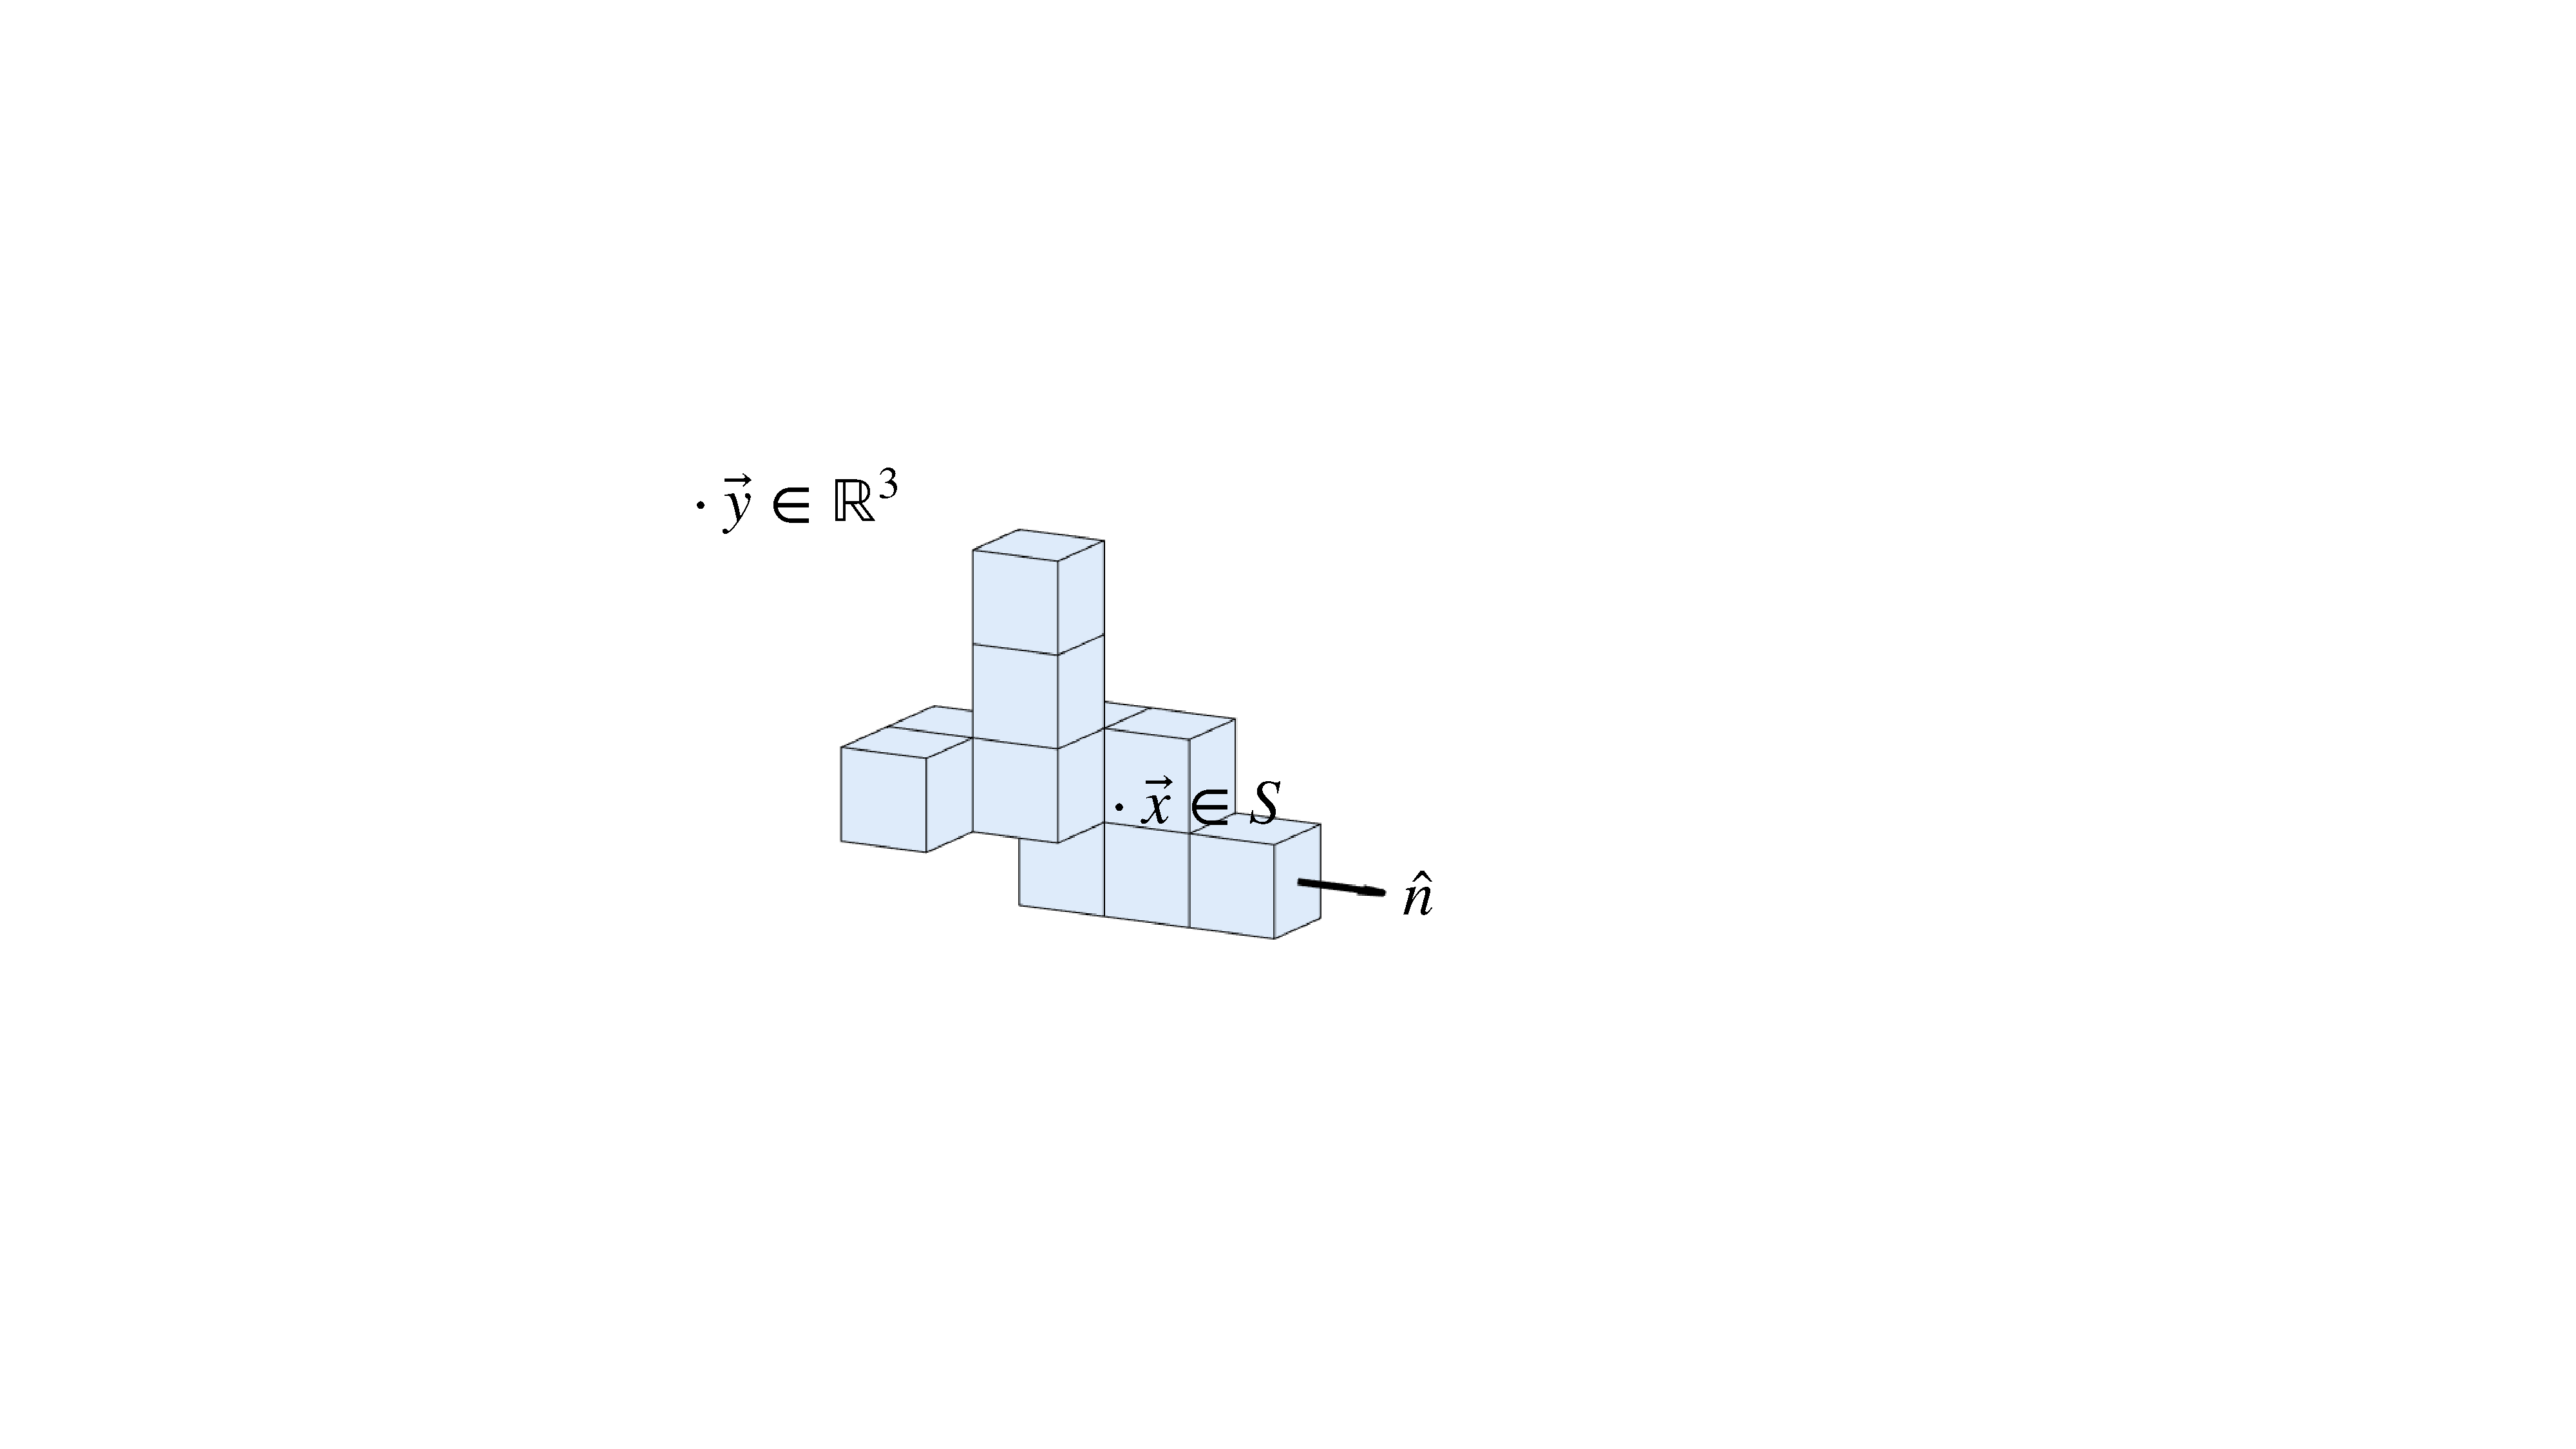
\includegraphics[scale=0.25]{figures/fig_sample_cube10.pdf}

	\caption{Example aggregate model with 10 cubes. We denote $S$ as the aggregate boundary surface and $\hat{n}$ as its normal. The vectors $\vec{x}$ and $\vec{y}$ are points on and outside of $S$. The solid lines represent the fluid domain boundaries. } 

\label{fig_cube10}
\end{center}
\end{figure}

\section{Fluid momentum equations}
To describe the incompressible fluid motion that takes place around marine aggregates, we consider the Navier-Stokes equations,
\begin{align}
\nabla \cdot \vec{u} = 0 
\label{eq_conserv_mass} \\
\rho 
\left( 
   \frac{\partial \vec{u}}{\partial t} + \vec{u}\cdot \nabla \vec{u}
\right)
  = \nabla \cdot \bar{\bar{\sigma}} +  \rho  \vec{g} ,
\label{eq_momentum_NS}
\end{align}
where $ \rho$ is fluid density (constant) and $\vec{u}, \ \vec{g}$ are fluid velocity and gravity vectors, respectively.
The first equation (\ref{eq_conserv_mass}) shows the conservation of mass and the equation (\ref{eq_momentum_NS}) describes the momentum conservation. 
We also introduce the stress tensor, $\bar{\bar{\sigma}}$ as sum of the fluid pressure $P$ and deviatoric stress tensor $\bm{\tau}$,
\begin{equation}
   \bar{\bar{\sigma}} =-P \bar{\bar{I}} + {\bm \tau} = -P \bar{\bar{I}} + {\tilde{\mu}} {\bm D},
   \label{eq_stress_tensor}
\end{equation}
where ${\tilde{\mu}}$ is constant fluid viscosity and ${\bm D}$ is the symmetric strain rate tensor, that is,
\begin{equation}
   \boldsymbol{D} = \frac{1}{2} \left( \nabla \vec{u} + {(\nabla  \vec{u} )}^T \right).
   \label{eq_strain_rate}
   \end{equation}
Since seawater is a Newtonian fluid, following Newton's law of viscosity, the strain rate (\ref{eq_strain_rate}) becomes $\nabla \vec{u}$. This implies that we can re-write the momentum equation (\ref{eq_momentum_NS}) as
\begin{equation}
  \rho \left( 
   \frac{\partial \vec{u}}{\partial t} + \vec{u}\cdot \nabla \vec{u}
\right)
  = -\nabla P  + {\tilde{\mu}} \nabla^2 \vec{u}+  \rho  \vec{g} 
  \label{eq_stokes_momentum}
\end{equation}
For a typical seawater, it is reasonable to say $\rho \approx 1025 \text{kg/m}^3$ and ${\tilde{\mu}} = 1.2 \times 10^{-3}\text{kg}/\text{ms}$.
Also, the gravitaty vector is $\vec{g} = - g\hat{k} \approx -9.8$m/$s^2 \times (0,0,1)$ where $\hat{k}$ points in the vertical direction (upward). 
\par
 The momentum equation (\ref{eq_momentum_NS}) can be linearized for flows where inertial effects are small. 
To estimate the size of the main forces at play, we consider a radius of marine aggregate, $R_a \approx 5 \times 10^{-5} (\text{m})$ and the reference Stokes settling speed of an aggregate,
\begin{equation}
    U_s =  \frac{gR_a^2}{{\tilde{\mu}}} (\rho_a-\rho) \approx 3.8 \times 10^{-4} ({\text{m/s}}),
	\label{eq_U_s}
\end{equation}
where $\rho_a \approx 1400\text{kg/m}^3$ is the aggregate mass density. 
When we non-dimensionalize the momentum equation using the length scale, $R_a$ and velocity, $U_s$, we can obtain the following equation:
\begin{equation}
	\left(\frac{\rho U_s R_a}{{\tilde{\mu}}} \right) 
   \left( 
   \frac{\partial \vec{u}'}{\partial t'} + \vec{u}'\cdot \nabla' \vec{u}'
\right)
 = {\nabla'}^2 \vec{u}' - \nabla' P' +  \vec{g}',
 \label{eq_NS_moment_noD}
\end{equation}
where we find and compute the Reynolds number (Re),
\begin{equation}
	\text{Re} = \frac{\rho U_s R_a}{{\tilde{\mu}}} \approx 10^{-2}
	\ll 1.
   \label{eq_Re}
\end{equation}
Note that we use the prime symbol to represent a dimensionless value.
Since we have a fairly small Reynolds number, we may neglect the inertial effects, limiting the left-hand side of the equation (\ref{eq_NS_moment_noD}) to zero,
\begin{equation}
   {\nabla'}^2 \vec{u}' - \nabla' P' +  \vec{g}' = 0.
\end{equation}
In this thesis, we, therefore, consider the following Stokes equations, writing back with dimensions, to describe the fluid flow around the settling aggregates,
 \begin{align}
	\nabla \cdot \vec{u}  = 0  
	% \label{eq_conti2}
	\nonumber \\
	{\tilde{\mu}} \nabla^2 \vec{u}    - \nabla P\ + \rho  \vec{g} = 0.
	\label{eq_stokes2}
\end{align}
The solutions of the system of equations are the fluid velocity, $\vec{u}$, and pressure, $P$. In general, pressure does not induce motion. We see the pressure at rest, denoted as $P_s$, contains the pressure of gravity,  $P_s(\vec{y}) = \rho \vec{g} \cdot \vec{y}$, where $\vec{y} \in \mathbb{R}^3$ is a point in the fluid. Using this static pressure term, we introduce the dynamic pressure $P_d$, defined as 
\begin{equation}
   P_d(\vec{y}) = P(\vec{y}) - P_s(\vec{y}) = P(\vec{y}) - \rho \vec{g} \cdot \vec{y}.
   \label{eq_def_Pd}
\end{equation}
By substituting the expression (\ref{eq_def_Pd}), we obtain
\begin{align}
	\nabla \cdot \vec{u}  = 0  
	% \label{eq_conti2}
	\nonumber \\
	{\tilde{\mu}} \nabla^2 \vec{u}    - \nabla P_d = 0.
	\label{eq_stokes3}
\end{align}
In our simulation, we focus on the velocity field and hydrodynamic forces around the marine aggregate model. 
%===SECTION 2.2=========================================
\section{Boundary integral equation (BIE) formulations} 
For our simulations, we consider a large fluid domain compared to the size of an aggregate, having zero fluid velocity at infinity. We also treat our aggregate surface as a solid. Although marine aggregates are porous, the solid boundary condition is reasonable to apply due to their low permeability. 
This condition prevents a flow through the aggregate, acting like a solid particle. For this reason, any flow inside of the aggregate is neglected in the remainder of this thesis.  
\par
For a general surface S, the velocity $\vec{u}$ at a point $\vec{y}\in \mathbb{R}^3$ exterior to the surface may generally be expressed using the representation formula~\cite{pozrikidis_boundary_1992}
% around a solid object is expressed, using the stress vector, $\vec{f}$, 
\begin{equation}
   \vec{u}(\vec{y}) =
	- \frac{1}{8 \pi {\tilde{\mu}}} \int_S  \vec{f}(\vec{x}) \cdot \bar{\bar{G}}(\vec{x},\vec{y}) \ \text{d}S(\vec{x}) 
+ \frac{1}{8 \pi} \int_S
\vec{u}(\vec{x}) \cdot  \bar{\bar{K}}(\vec{x},\vec{y})  
\cdot \hat{n} ( \vec{x})
\ \text{d}S(\vec{x}),
\label{eq_BIE}
\end{equation}
% where  $\vec{f}(\vec{x})$ is the stress vector that describes a point force at $\vec{x} \in S$. 
where the integral is taken over points $\vec{x}$ on the surface $S$.
The kernel $\bar{\bar{G}}(\vec{x},\vec{x}_0)$ is the Green's function of the Stokes equations at any point $\vec{y}$, that is the {\textit{Stokeslet}}, in the domain for a point-source located at $\vec{x}$,
\begin{align}
  \bar{\bar{G}}(\vec{x},\vec{y}) =   
  \frac{\bar{\bar{I}}}{||\vec{x}-\vec{y}||} + \frac{(\vec{x}-\vec{y})(\vec{x}-\vec{y})}{||\vec{x}-\vec{y}||^3}.
  \label{eq_stokeslet}
  \end{align}
  The kernel  $\bar{\bar{K}}(\vec{x},\vec{y})$ is the stress tensor associated with this fundamental solution, named {\textit{Stresslet}},
  %
  \begin{align}
  \bar{\bar{K}}(\vec{x},\vec{y}) = 
  -6\frac{(\vec{x}-\vec{y})(\vec{x}-\vec{y}) (\vec{x}-\vec{y})}{||\vec{x}-\vec{y}||^5},
  \label{eq_stresslet}
  \end{align}
where $\| \cdot \|$ is the $L^2$ norm. 
The first integral distribution on the right-hand side of the equation (\ref{eq_BIE}) is called the \textit{single-layer potential} and the second one is called the \textit{double-layer potential}. 
To compute the velocity at a point on the surface $S$, i.e., $ \vec{x}_s \in S$, we use 
\begin{equation}
   \vec{u}(\vec{x}_s) = - \frac{1}{4 \pi {\tilde{\mu}}} \int_S  \vec{f}(\vec{x}) \cdot \bar{\bar{G}}(\vec{x},\vec{x}_s) \ \text{d}S(\vec{x}) 
+ \frac{1}{4 \pi} 
\int_S
\vec{u}(\vec{x}) \cdot  \bar{\bar{K}}(\vec{x},\vec{x}_s)  
\cdot \hat{n} ( \vec{x})
\ \text{d}S(\vec{x}).
\label{eq_BIE_onS}
\end{equation}
Also, $\vec{f}(\vec{x})$ is the generally unknown stress vector, or traction, on the surface, and $\vec{u}(\vec{x})$ is the, generally unknown, velocity on the surface $S$. 
When $S$ is the boundary of a solid object, in our case an aggregate, the general representation formula may be simplified in two different ways, depending on the fluid domain characteristics and/or type of the object's surface. We will introduce those two formulae in Chapter 2. 


\section{Non-Newtonian fluid}
In the last part of this thesis, we will turn our attention to non-Newtonian fluids. This topic is added to my thesis as an extension of one summer internship at the Lawrence Berkeley National Lab in 2022, under the guidance of Dr.Ishan Srivastava. 
\par
A non-Newtonian fluid shows many interesting behaviors quite different than Newtonian fluids. The major difference we focus on here is the viscous stress tensor, $\bar{\bar{\sigma}}$. The viscosity term, which is part of $\bm{\tau}$ in equation (\ref{eq_stress_tensor}), is not constant anymore; rather it is a function of the shear rate $\dot{\gamma} = \left| {\boldsymbol{D}} \right|$.
Due to this varying viscosity, the constitutive behavior of non-Newtonian fluids is highly complex. 
\par
They show intriguing phenomena such as shear thickening, shear thinning, and jamming. Figure \ref{fig_rheology} shows an idea of those different behaviors depending on the relationships between shear stress and rate. 

This broad class of fluids encompasses various materials of industrial and natural importance, such as granular fluids, polymeric fluids, gels, and suspensions. Complex fluids exhibit two phases as responses to applied stress and the study for this fluid type is called {\textit{rheology}}. 
% As the viscosity of a non-Newtonian fluid can be a function of the shear rate, a defining feature of many complex fluids is the presence of yield stress: for an insufficiently stressed material, they behave like an elastic solid, but once the yield stress is exceeded, they flow like a fluid. 
\begin{figure}[h]
	\begin{center}
		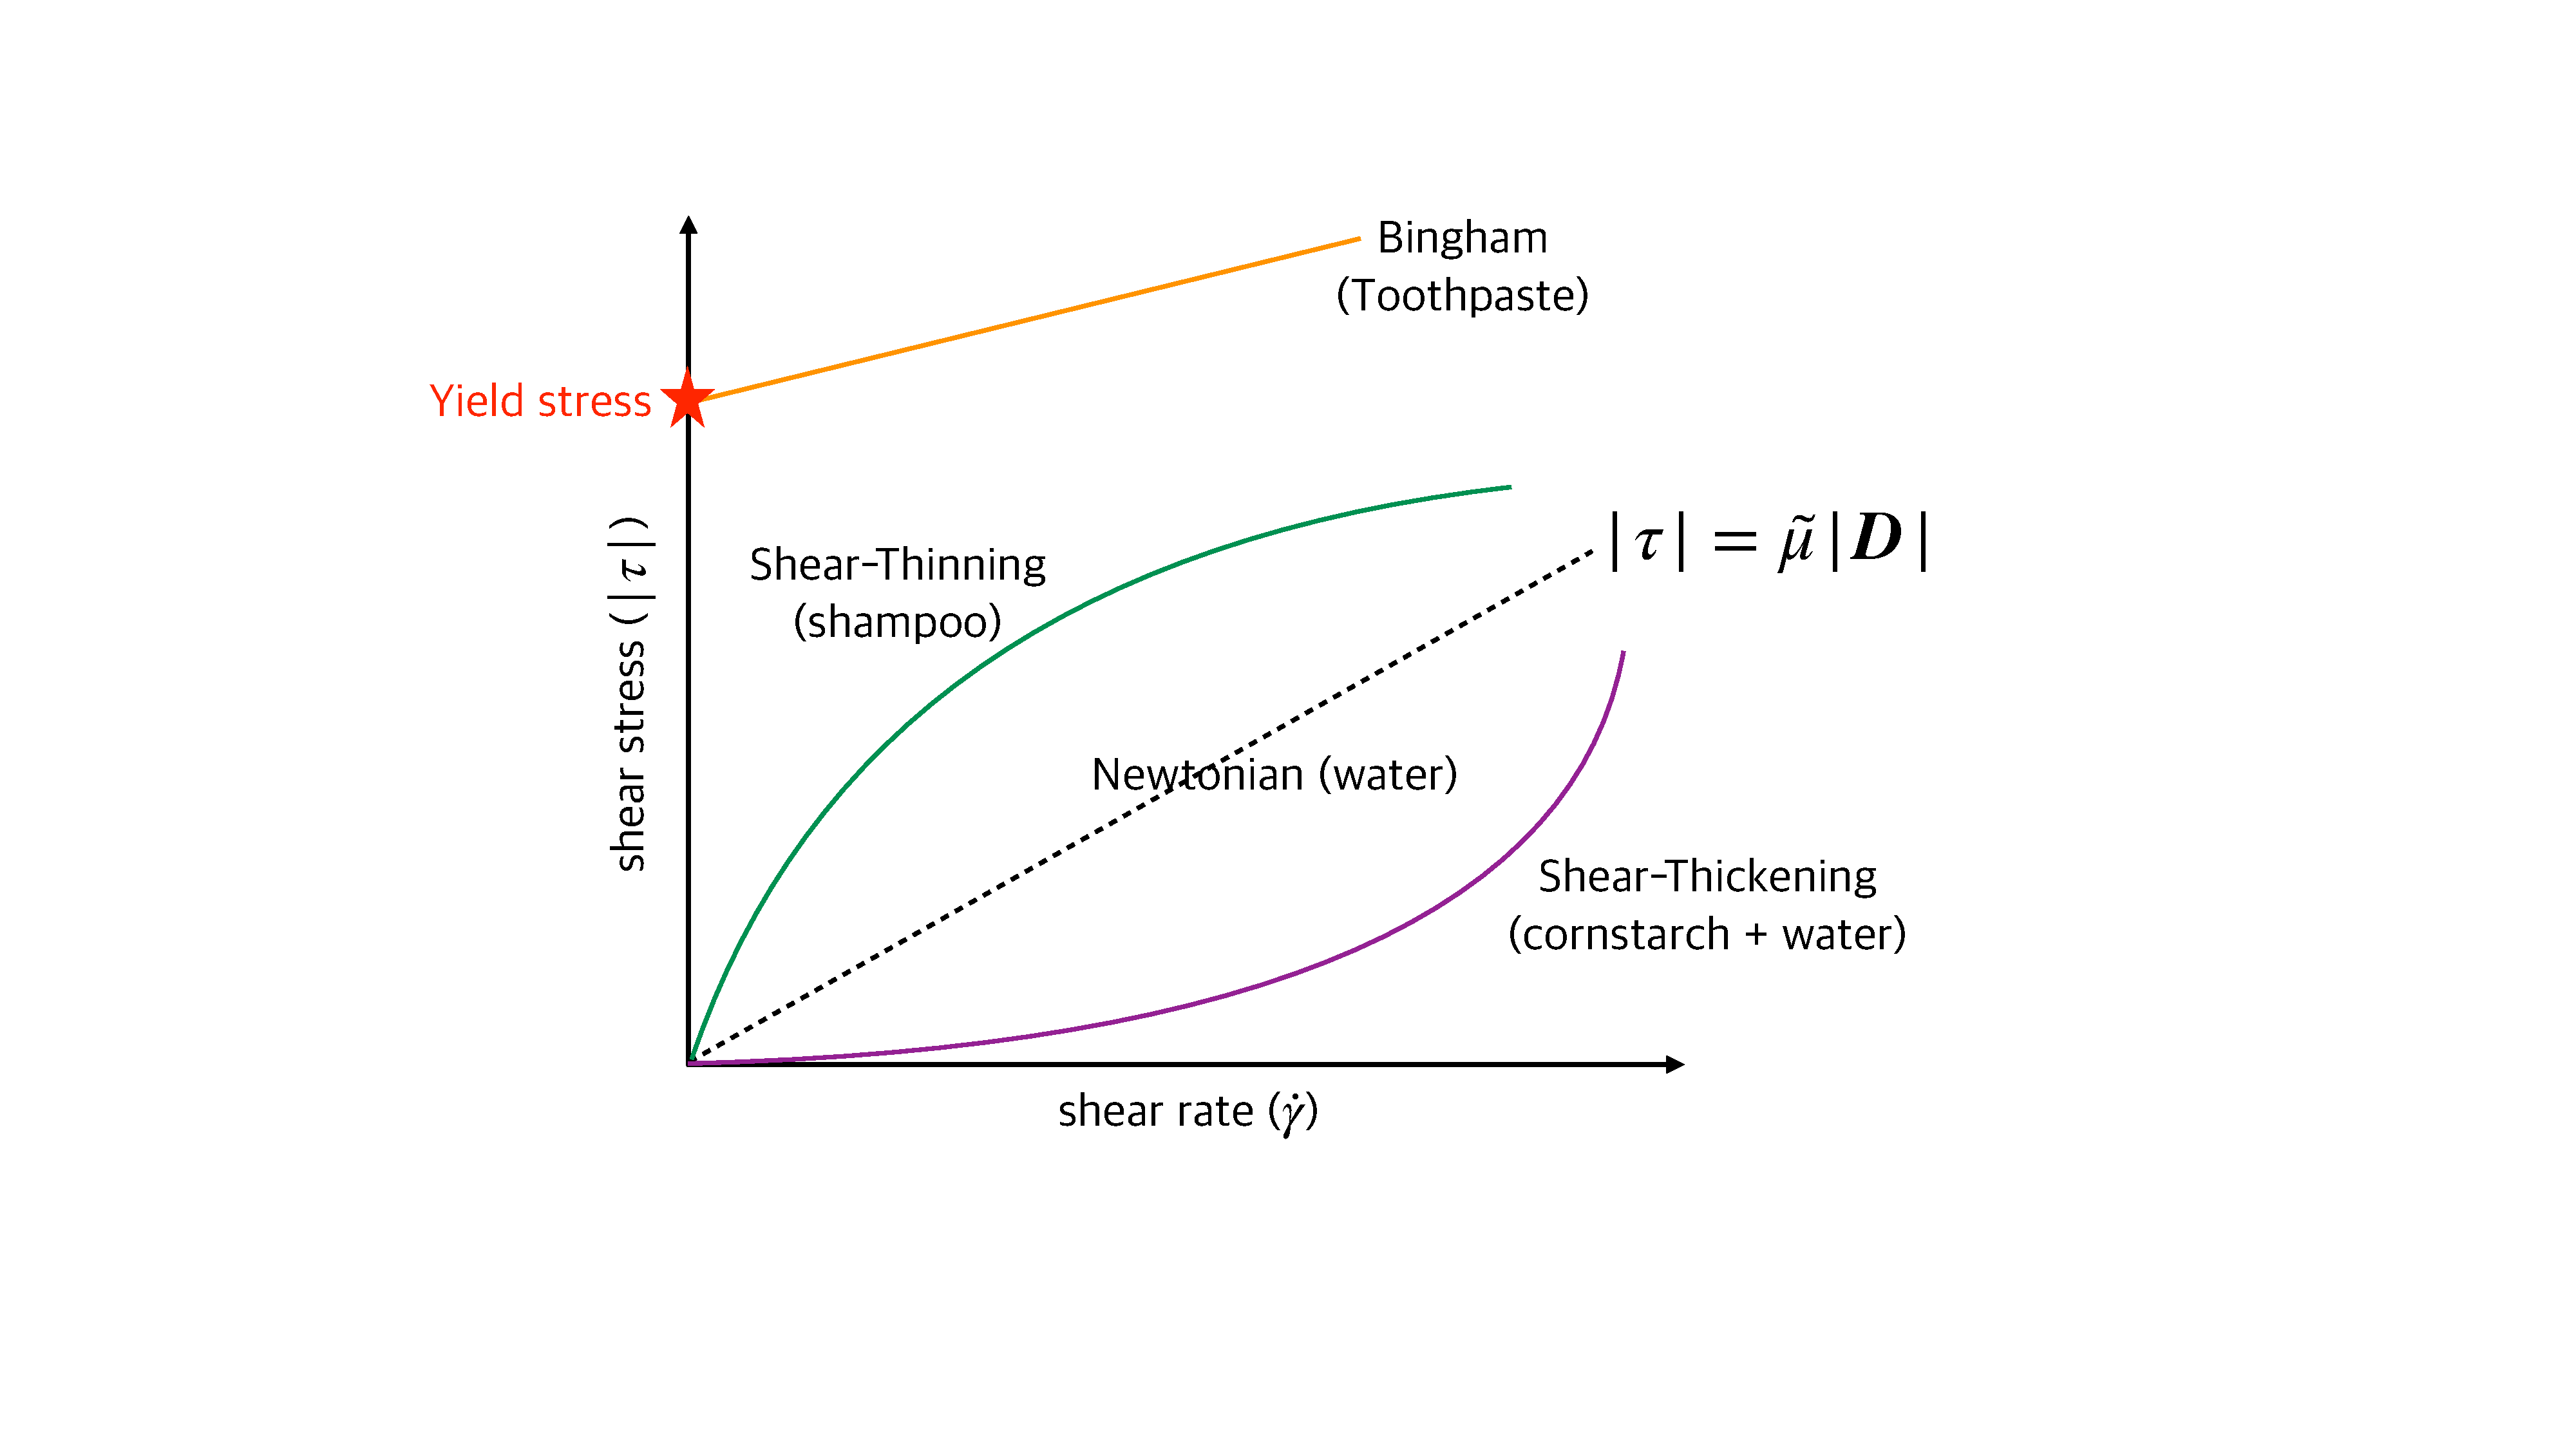
\includegraphics[scale=0.25]{figures/fig_yield_stress_graph.pdf}
	\end{center}
   \caption{Solid lines show different types of non-Newtonian behavior with examples in the parenthesis. The red star describes yield stress. The dashed line represents Newton's law of viscosity.}
\label{fig_rheology}
\end{figure}
\par
From the Cauchy stress tensor, showing its explicit form, 
\begin{equation}
  \bar{\bar{\sigma}} = 
  \begin{bmatrix}
    \sigma_{xx} & \sigma_{xy} & 0 
    \\
    \sigma_{xy} & \sigma_{yy} & 0 
    \\
    0 & 0 & \sigma_{zz},
  \end{bmatrix}
  \label{eq_cauchy_mx}
\end{equation} 
we define the first normal stress difference $N_1$
\begin{equation}
  N_1 = \sigma_{xx} - \sigma_{yy}
\end{equation}
and the second normal stress difference $N_2$,
\begin{equation}
  N_2 = \sigma_{yy} - \sigma_{zz}.
\end{equation}
Unlike a Newtonian case having $N_1 = N_2 = 0$, we can observe $\sigma_{xx} \neq \sigma_{yy} \neq \sigma_{zz}$ for a non-Newtonian fluid in shear flows.
To describe a non-Newtonian flow behavior, the deviatoric stress tensor requires a higher-order relationship with the strain rate tensor $\bm{D}$. The following form is introduced by Colemann and Noll~\cite{coleman_approximation_1960} with complexity order 2,
\begin{equation}
   \boldsymbol{\tau} = \nu_1 {\bm A_1} + \alpha_1 {\bm A_2} + \alpha_2 {\bm A_1^2},
   \label{eq_CN_tau}
\end{equation}
where $\nu_1$ is the constant viscosity and $\alpha_i = N_i / \dot{\gamma}$ for $i = 1,  2$.
The $\bm{A_i}$ are called Rivlin-Ericksen tensors defined by
\begin{equation}
   {\bm A_1}  = \nabla \vec{u} +  \left( \nabla \vec{u} \right)^T = 2 \bm{D}
\end{equation}
and 
\begin{equation}
   \boldsymbol{A}_2
   % =\frac{D}{D t} \boldsymbol{A}_1+\boldsymbol{A}_1 \nabla \vec{u}+ \left(\nabla \vec{u} \right)^T \boldsymbol{A}_1
   =\frac{\partial \boldsymbol{A}_1}{\partial t} + \vec{u} \cdot \nabla \boldsymbol{A}_1+\boldsymbol{A}_1 \nabla \vec{u}+ \left(\nabla \vec{u} \right)^T \boldsymbol{A}_1
\end{equation}
One may notice that many researchers did not include the effect of $\bm{A_1}^2$. For polymer solutions, the most studied in the complex fluids field, it is well-known that $N_2$ is small enough to ignore, compared to $N_1$~\cite{bird_dynamics_1987}. However, there are potentially important characteristics that are neglected when we consider the stress linear in $\boldsymbol{D}$ only. For instance, curvature in free-surface flows~\cite{couturier_suspensions_2011}, anomalous stress profile in cylindrical Couette flows~\cite{krishnaraj_dilation-driven_2016}, or negative rod climbing effect (Weissenberg effect)~\cite{boyer_dense_2011}. We thus want to implement computational tools to study these normal stress differences. 
% \begin{align}
% \bar{\bar{\sigma}}
%   = -P \bar{\bar{I}}  + \ &\mu_1 {\bm D} 
%   + \mu_2  \left[ {\bm D}^2  - \frac{\text{tr}\left({\bm D}^2\right)}{3}{\bm I} \right]
% + \kappa_1 \frac{{\bm D}}{|{\bm D}|} 
%   + \kappa_2  \left[ \frac{{\bm D}^2}{|{\bm D}|^2}  
%   - \frac{\text{tr}\left({\bm D}^2\right)}{3|{\bm D}|^2}{\bm I} \right].
% \label{eq_sigma_noN}
% \end{align}
% The terms $\mu_i, \kappa_i > 0 $ ($i, j = 1,2$) coefficients represent the shear rate-dependent and rate-independent contributions, respectively, to the total stress.
\par
With a constitutive rheology code, we can capture such complex continuum hydrodynamics. 
We work on the \href{https://amrex-codes.github.io/index.html}{{\color{blue}AMReX-Codes}}, which is a block-Structured Adaptive Mesh Refinement (AMR) Software Framework and Applications. In Summer 2022, following Dr. Strastava's guidance, we focused on granular rheology, implementing the particular viscosity term, by considering both the shear rate and external pressure, in an individual module of AMReX called \textit{incflo}. 
\par
As a first step, we connect the granular rheology code to an incompressible flow model, assuming a steady state. To solve an incompressible flow velocity using equations (\ref{eq_conserv_mass}) and (\ref{eq_momentum_NS}), it is necessary to evaluate the divergence of the stress tensor, $\nabla \cdot \bar{\bar{\sigma}}$. Once we have the stress tensor of the form (\ref{eq_CN_tau}), which is non-linear in velocity, it becomes numerically complicated to solve the Navier-Stokes equations. The most convenient choice of time integration would be an explicit method. However, it is not the best option, considering stability and efficiency. In incflo, at the moment I was interning, there were three integrations were available: 1) Explicit Euler, 2) Crank-Nicolson, and 3) implicit Euler methods. 
% We thus consider both the shear stress rate and the pressure onto the materials of interest as the sources of the yield stress. 




